%% A 3-page report describing the central aspects of your A* program, such as
% the agenda and how it is managed. This must clearly and concisely document
% the generality of your program: it should illustrate how your program can
% easily be reused on other search tasks, with only a little subclassing needed
%for each new task. So the core code should NOT have details specific to the
% navigation task. The report must also describe your heuristic function and
% your method for generating successor states. The report must NOT exceed 3
% pages, including all diagrams, code segments, etc. (4 points)
\section{Central aspects of your A* program}
\subsection{The agenda and how it is managed}
The agenda is awesome. list and Heapq\ldots

\subsection{Generality of the program}

\begin{figure}[h!]
	\centering
	\resizebox {!} {8cm} {
		\begin{tikzpicture} 
			\umlclass{BestFirstSearch}{
				start : SearchState
			}{
				+ attach\_and\_eval(child : SearchState, parent : SearchState) : void \\
				+ propagate\_path\_improvements(parent : SearchState) : void \\
				+ best\_first\_search() : SearchState \\
				+ \umlvirt{arc\_cost(a : SearchState, b : SearchState) : double} \\
				+ \umlvirt{create\_root\_node() : SearchState} \\
				+ open\_push(opened : [], node : SearchState) : void \\
				+ open\_pop(opened : []) : SearchState \\
				+ node\_closed(node : SearchState, t\_0 : long, generated : {}, opened : [], closed : []) : void
			}
			\umlclass[right=13cm of BestFirstSearch.north, anchor=north]{SearchState}{
				state : object \\
				sid : string \\
				status : int \\
				parent : SearchState \\
				kids : [] \\
				g : double \\
				h : double \\
				f : double
			}{
				+ add\_child(child : SearchState) : void \\
				+ \umlvirt{create\_state\_identifier() : string} \\
				+ \umlvirt{heuristic\_evaluation() : double} \\
				+ \umlvirt{is\_solution() : boolean} \\
				+ \umlvirt{solution\_length() : double} \\
				+ \umlvirt{generate\_all\_successors() : SearchState}
			}
			\umlclass[below=8cm of SearchState.north, anchor=north]{NavigationState}{
				visited : [] \\
				current\_pos : []
			}{
				+ create\_state\_identifier() : string \\
				+ heuristic\_evaluation() : double \\
				+ is\_solution() : boolean \\
				+ solution\_length() : double \\
				+ generate\_all\_successors() : SearchState \\
				+ euclidean\_distance(a : [], b : []) : double \\
				+ manhattan\_distance(a : [], b : []) : double \\
				+ print\_level() : void
			}
			\umlclass[below=6cm of BestFirstSearch.north, anchor=north]{NavigationBfs}{}{
				+ arc\_cost(a : SearchState, b : SearchState) : double \\
				+ create\_root\_node() : SearchState
			}
			\umlinherit[geometry=-|, anchors=north and south]{NavigationState}{SearchState}
			\umlinherit[geometry=-|, anchors=north and south]{NavigationBfs}{BestFirstSearch}
			\umlunicompo[geometry=-|, stereo=start, anchors=east and 164, pos stereo=0.5]{BestFirstSearch}{SearchState}
		\end{tikzpicture}
	}
	\caption{Class diagram for the navigation task.}
\end{figure}

Figure \ref{run:ex5} shows the class diagram for the navigation problem.

\lstinputlisting[emph={HelloWorldPrintable}]{module_1/code_snippets/hello_world.py}

\subsection{Heuristics}
Both the \emph{Manhattan distance} and \emph{Euclidean distance} has been tested on the navigation problem. Each adjusted the behaviour of the agent. Using the manhattan distance the agent seem preferring to minimize the amount of \(90 deg\) turns before reaching the final goal. The euclidean distance seems to do the quite opposite, and the agent goes straight towards the target even though the agent cannot move diagonally. It tries to emulate the behaviour of walking diagonally and follows a diagonal line between the current position and the goal. In the example board number two (Figure \ref{run:ex2}), the manhattan distance wins by generating least amount of nodes, because it can just move right and then up without encounter an obstacle. The euclidean agent has to avoid an obstacle and therefore is generating a few more nodes. On the other hand, in example 5 (Figure \ref{run:ex5}), the euclidean agent slips through the opening between the two last obstacles, while the manhattan agent needs to explore the area before the right-most obstacle. The performance of the agent depends on the heuristics compared with the structure of the board.

\begin{figure}[h!]
	\centering
	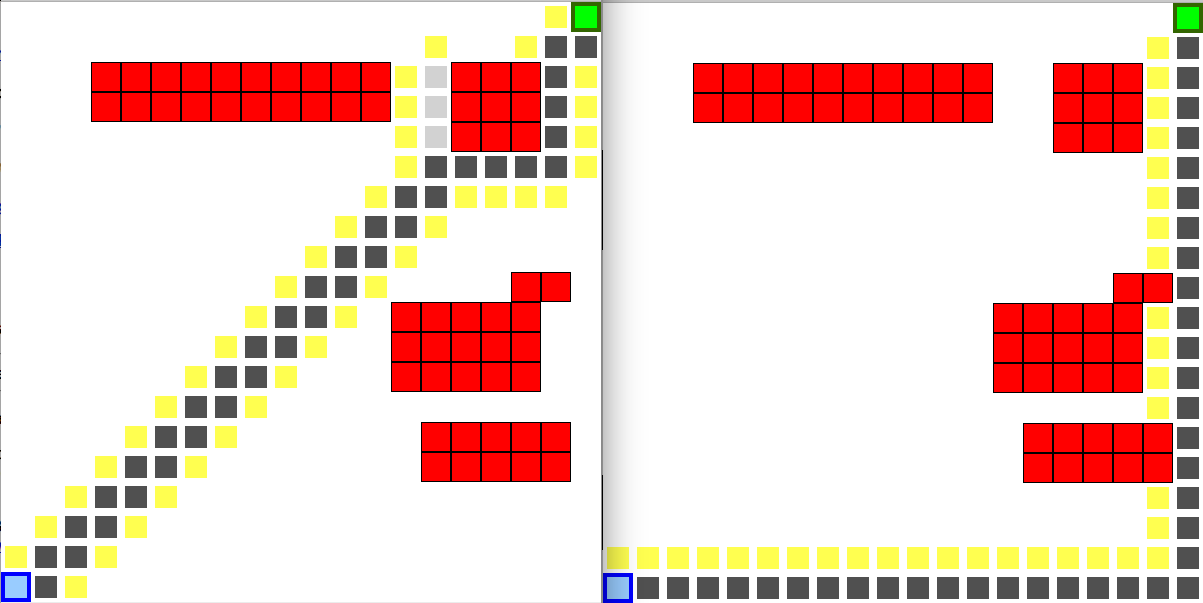
\includegraphics[width=0.8\textwidth]{module_1/images/run_ex2}
	\caption{Comparing euclidian distance and manhattan distance in board example 2}
	\label{run:ex2}
\end{figure}

\begin{figure}[h!]
	\centering
	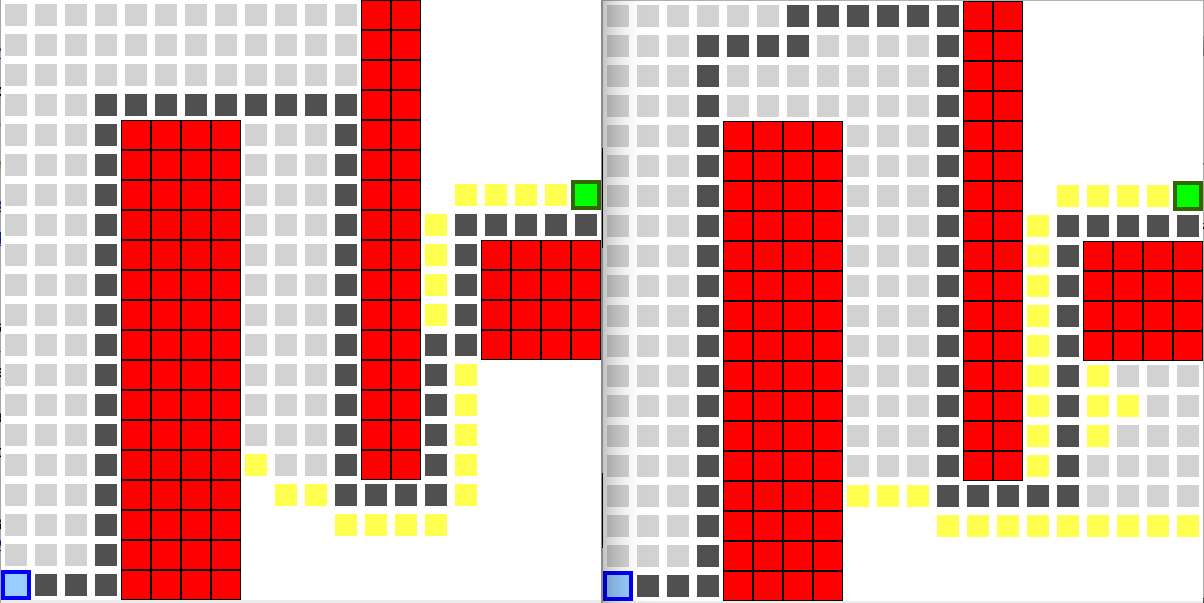
\includegraphics[width=0.8\textwidth]{module_1/images/run_ex5}
	\caption{Comparing euclidian distance and manhattan distance in board example 5}
	\label{run:ex5}
\end{figure}

\subsection{Generating successor states}
From each viable state, a maximum of four possible successor states can be created, each by moving in every direction from its currently held position; NORTH, SOUTH, EAST, WEST. Other considered limitations are that the new position should be inside the given dimensions of the board, and that obstacles are not walkable, together with unnecessity to visit positions that previously have been visited. Every state that is within the scope of those limitations, is created and added to the heap.